\section{Développement de l'application}

L'application finale demandée reprend les éléments de configuration vus en section 2.
Cette section comporte un récapitulatif des éléments de l'application avec éventuellement des portions de code montrant leur utilisation.
Un exemple de résultats obtenus après lancement de l'application sont montrés;

\subsection{Éléments de l'application}

L'application se base sur la structure fonctionnelle suivante:

\begin{figure}[h]
    \centering
    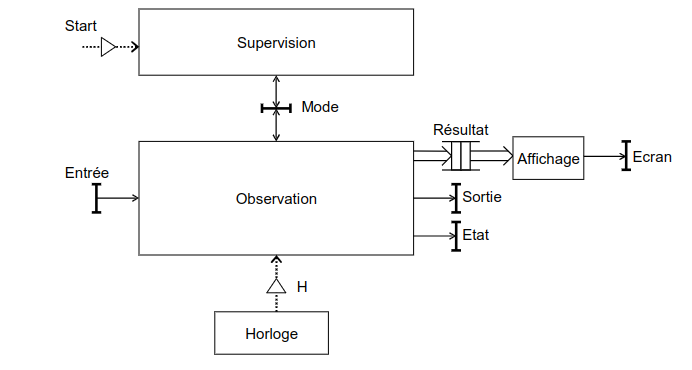
\includegraphics[width=0.7\linewidth]{struct_fonc.png}
    \caption{Structure fonctionnelle de l'application à développer}
    \label{fig:struct}
\end{figure}

De ce schéma, différentes informations peuvent être extraites.
Quatre tâches distinctes peuvent être imaginées pour cette application temps-réel:

\begin{itemize}
    \item Horloge
    \item Supervision
    \item Observation    
    \item Affichage
\end{itemize}

Nous pouvons faire l'hypothèse que deux sémaphores, matérialisées dans la structure par les relations de Start et H, peuvent être implantées au sein de l'application.
L'application contient une variable partagée \textit{Mode} et une file de message \textit{Résultats}.
Les différentes entrées/sorties présentées dans cette structure fonctionnelle correspondent à des éléments physiques présents sur la carte tels que des boutons poussoirs, des LEDs ou l'écran.

\subsection{Résultat}

L'application peut être testée en programmant la carte.
L'utilisateur doit appuyer sur le bouton SW0 pour lancer une série de mesure du temps de réaction.
Dans le cadre des résultats montrés ci-dessous, cinq mesures successives sont effectuées avant l'affichage des résultats sur l'écran.
Les figures suivantes montrent l'affichage de l'écran au lancement de l'application (\ref{fig:start_app}) et à la fin d'une série de mesure (\ref{fig:end_app}).
Les résultats montrés sont, dans l'ordre:

\begin{itemize}
    \item Le temps de réaction minimal
    \item Le temps de réaction moyen
    \item Le temps de réaction maximal
    \item La période d'observation entre deux appels de la tâche Observation
\end{itemize}

L'unité de chacune de ces valeurs est le \textit{tick d'horloge}.
Le projet utilise une horloge à la fréquence de 8 MHz, divisée par un facteur AAA.
Ainsi, un \textit{tick d'horloge} correspond à approximativement BBB secondes.

\begin{figure}[h]
    \centering
    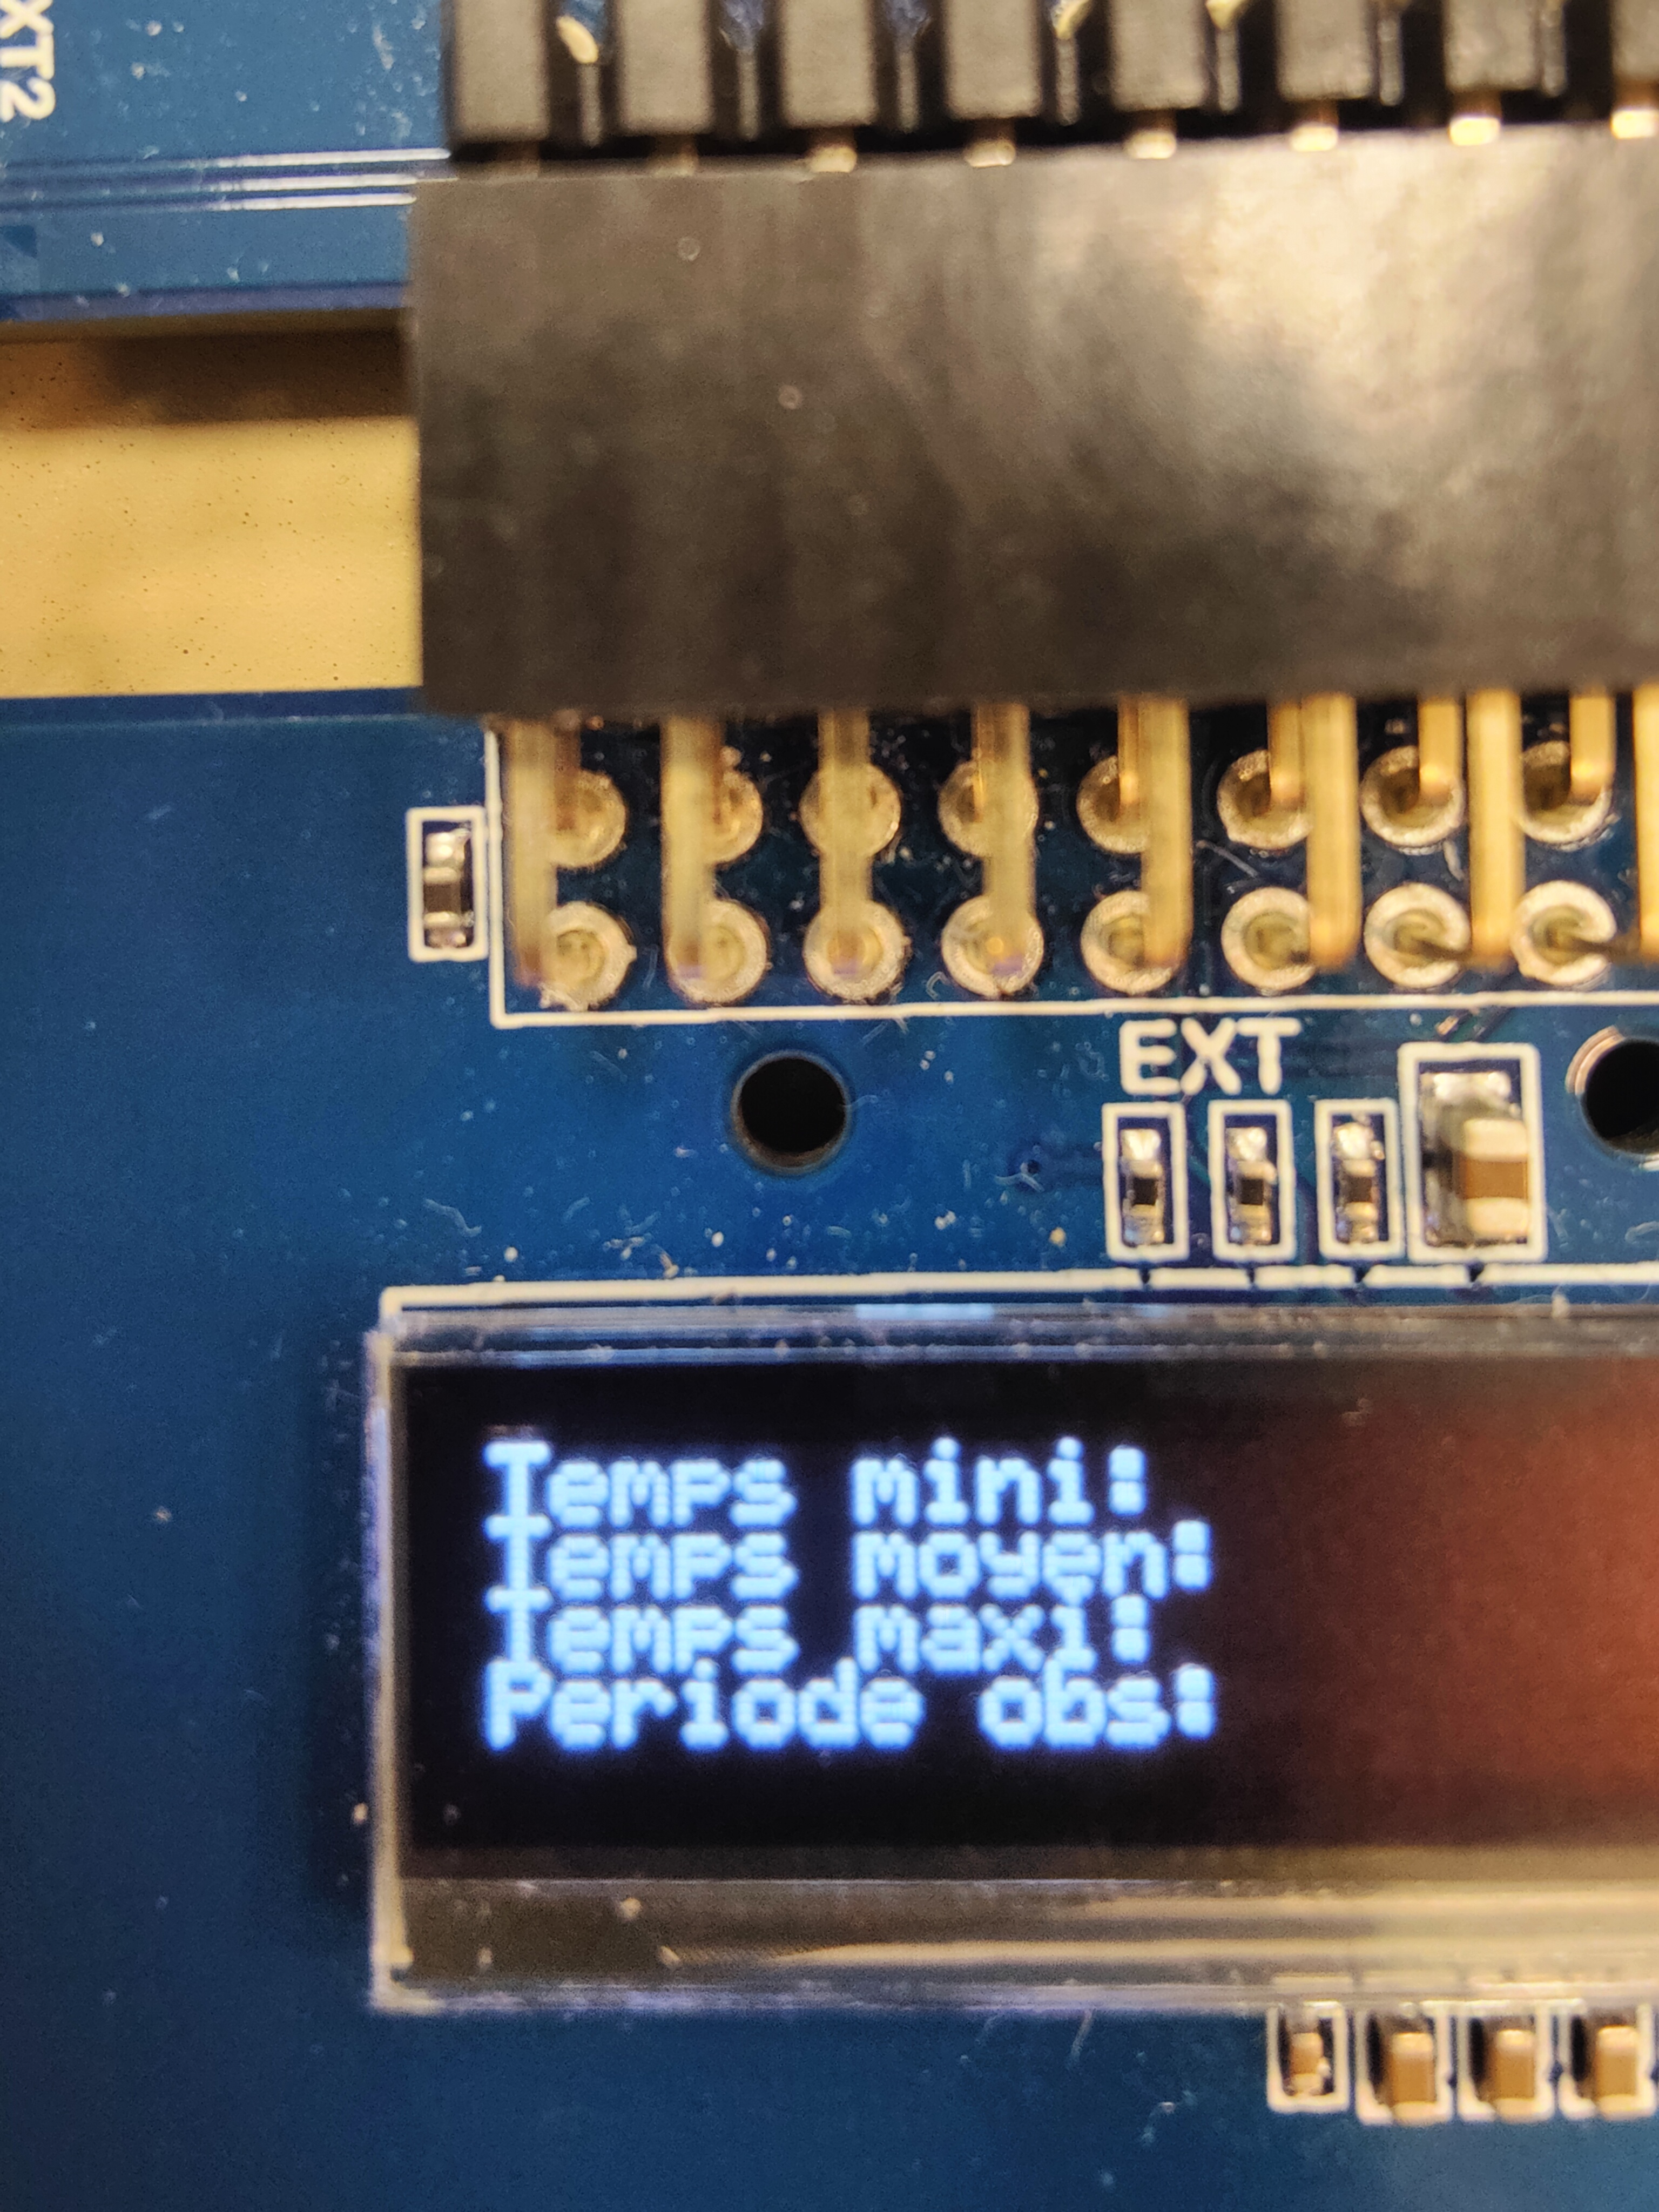
\includegraphics[width=0.4\linewidth]{start_app.jpg}
    \caption{Affichage de l'écran au lancement de l'application}
    \label{fig:start_app}
\end{figure}

Au lancement de l'application, l'écran affiche du texte en préparation de l'arrivée des résultats.
C'est lors de l'initialisation du matériel que cet affichage a lieu.

\begin{figure}[h]
    \centering
    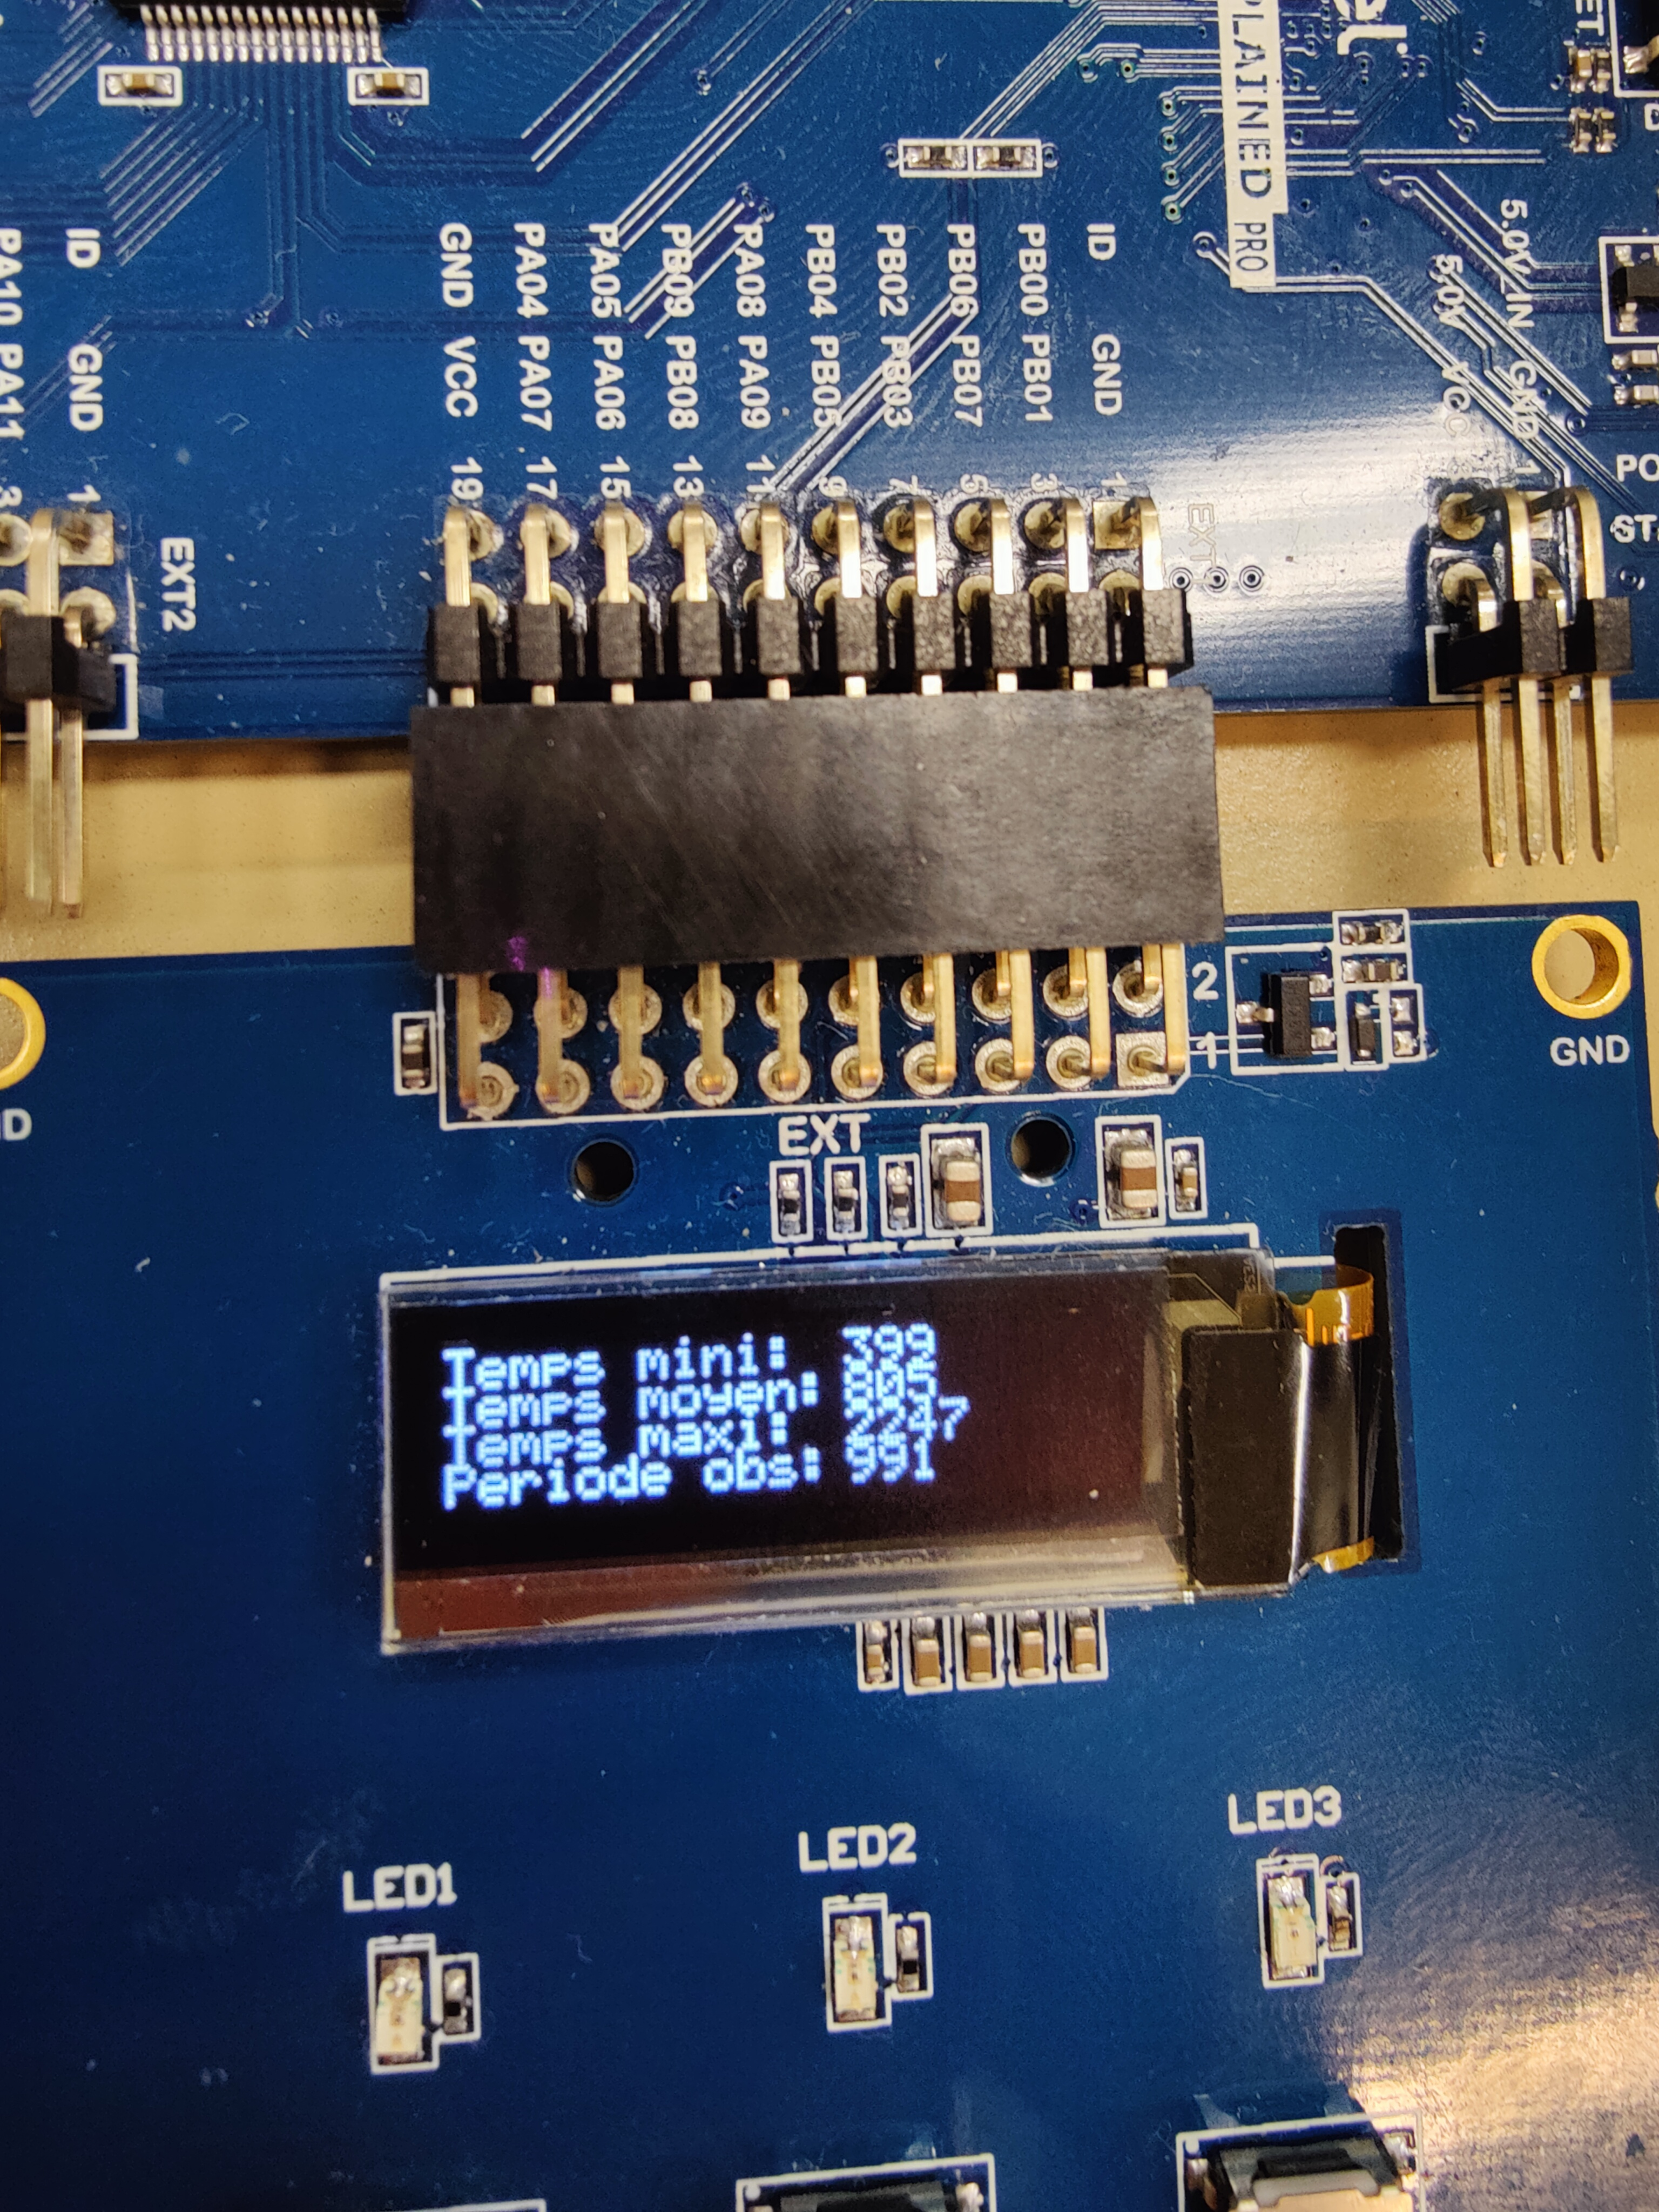
\includegraphics[width=0.4\linewidth]{end_app.jpg}
    \caption{Affichage de l'écran après une session de mesure du temps de réaction}
    \label{fig:end_app}
\end{figure}

Après une série de mesure, la file de message contenants les résultats est envoyée de la tâche \textit{Observation} à la tâche \textit{Affichage}.
Cette file de message contient la variable Résultat, instance de la structure \textit{Resultat\_t} contenant les différentes mesures.
Après réception de la file de message, la tâche \textit{Affichage} fait apparaître sur l'écran les résultats de la mesure.
\\\\
Pour prouver le bon fonctionnement de l'application, une vidéo est proposée dans le même dossier que ce rapport.
Cette vidéo couvre le démarrage de l'application après un reset. 
Une série de mesure a lieu, menant à l'affichage des résultats.
Enfin, l'utilisateur relance une série de mesure après appui sur le bouton SW0.